% Options for packages loaded elsewhere
\PassOptionsToPackage{unicode}{hyperref}
\PassOptionsToPackage{hyphens}{url}
\documentclass[
]{book}
\usepackage{xcolor}
\usepackage{amsmath,amssymb}
\setcounter{secnumdepth}{5}
\usepackage{iftex}
\ifPDFTeX
  \usepackage[T1]{fontenc}
  \usepackage[utf8]{inputenc}
  \usepackage{textcomp} % provide euro and other symbols
\else % if luatex or xetex
  \usepackage{unicode-math} % this also loads fontspec
  \defaultfontfeatures{Scale=MatchLowercase}
  \defaultfontfeatures[\rmfamily]{Ligatures=TeX,Scale=1}
\fi
\usepackage{lmodern}
\ifPDFTeX\else
  % xetex/luatex font selection
\fi
% Use upquote if available, for straight quotes in verbatim environments
\IfFileExists{upquote.sty}{\usepackage{upquote}}{}
\IfFileExists{microtype.sty}{% use microtype if available
  \usepackage[]{microtype}
  \UseMicrotypeSet[protrusion]{basicmath} % disable protrusion for tt fonts
}{}
\makeatletter
\@ifundefined{KOMAClassName}{% if non-KOMA class
  \IfFileExists{parskip.sty}{%
    \usepackage{parskip}
  }{% else
    \setlength{\parindent}{0pt}
    \setlength{\parskip}{6pt plus 2pt minus 1pt}}
}{% if KOMA class
  \KOMAoptions{parskip=half}}
\makeatother
\usepackage{color}
\usepackage{fancyvrb}
\newcommand{\VerbBar}{|}
\newcommand{\VERB}{\Verb[commandchars=\\\{\}]}
\DefineVerbatimEnvironment{Highlighting}{Verbatim}{commandchars=\\\{\}}
% Add ',fontsize=\small' for more characters per line
\usepackage{framed}
\definecolor{shadecolor}{RGB}{248,248,248}
\newenvironment{Shaded}{\begin{snugshade}}{\end{snugshade}}
\newcommand{\AlertTok}[1]{\textcolor[rgb]{0.94,0.16,0.16}{#1}}
\newcommand{\AnnotationTok}[1]{\textcolor[rgb]{0.56,0.35,0.01}{\textbf{\textit{#1}}}}
\newcommand{\AttributeTok}[1]{\textcolor[rgb]{0.13,0.29,0.53}{#1}}
\newcommand{\BaseNTok}[1]{\textcolor[rgb]{0.00,0.00,0.81}{#1}}
\newcommand{\BuiltInTok}[1]{#1}
\newcommand{\CharTok}[1]{\textcolor[rgb]{0.31,0.60,0.02}{#1}}
\newcommand{\CommentTok}[1]{\textcolor[rgb]{0.56,0.35,0.01}{\textit{#1}}}
\newcommand{\CommentVarTok}[1]{\textcolor[rgb]{0.56,0.35,0.01}{\textbf{\textit{#1}}}}
\newcommand{\ConstantTok}[1]{\textcolor[rgb]{0.56,0.35,0.01}{#1}}
\newcommand{\ControlFlowTok}[1]{\textcolor[rgb]{0.13,0.29,0.53}{\textbf{#1}}}
\newcommand{\DataTypeTok}[1]{\textcolor[rgb]{0.13,0.29,0.53}{#1}}
\newcommand{\DecValTok}[1]{\textcolor[rgb]{0.00,0.00,0.81}{#1}}
\newcommand{\DocumentationTok}[1]{\textcolor[rgb]{0.56,0.35,0.01}{\textbf{\textit{#1}}}}
\newcommand{\ErrorTok}[1]{\textcolor[rgb]{0.64,0.00,0.00}{\textbf{#1}}}
\newcommand{\ExtensionTok}[1]{#1}
\newcommand{\FloatTok}[1]{\textcolor[rgb]{0.00,0.00,0.81}{#1}}
\newcommand{\FunctionTok}[1]{\textcolor[rgb]{0.13,0.29,0.53}{\textbf{#1}}}
\newcommand{\ImportTok}[1]{#1}
\newcommand{\InformationTok}[1]{\textcolor[rgb]{0.56,0.35,0.01}{\textbf{\textit{#1}}}}
\newcommand{\KeywordTok}[1]{\textcolor[rgb]{0.13,0.29,0.53}{\textbf{#1}}}
\newcommand{\NormalTok}[1]{#1}
\newcommand{\OperatorTok}[1]{\textcolor[rgb]{0.81,0.36,0.00}{\textbf{#1}}}
\newcommand{\OtherTok}[1]{\textcolor[rgb]{0.56,0.35,0.01}{#1}}
\newcommand{\PreprocessorTok}[1]{\textcolor[rgb]{0.56,0.35,0.01}{\textit{#1}}}
\newcommand{\RegionMarkerTok}[1]{#1}
\newcommand{\SpecialCharTok}[1]{\textcolor[rgb]{0.81,0.36,0.00}{\textbf{#1}}}
\newcommand{\SpecialStringTok}[1]{\textcolor[rgb]{0.31,0.60,0.02}{#1}}
\newcommand{\StringTok}[1]{\textcolor[rgb]{0.31,0.60,0.02}{#1}}
\newcommand{\VariableTok}[1]{\textcolor[rgb]{0.00,0.00,0.00}{#1}}
\newcommand{\VerbatimStringTok}[1]{\textcolor[rgb]{0.31,0.60,0.02}{#1}}
\newcommand{\WarningTok}[1]{\textcolor[rgb]{0.56,0.35,0.01}{\textbf{\textit{#1}}}}
\usepackage{longtable,booktabs,array}
\usepackage{calc} % for calculating minipage widths
% Correct order of tables after \paragraph or \subparagraph
\usepackage{etoolbox}
\makeatletter
\patchcmd\longtable{\par}{\if@noskipsec\mbox{}\fi\par}{}{}
\makeatother
% Allow footnotes in longtable head/foot
\IfFileExists{footnotehyper.sty}{\usepackage{footnotehyper}}{\usepackage{footnote}}
\makesavenoteenv{longtable}
\usepackage{graphicx}
\makeatletter
\newsavebox\pandoc@box
\newcommand*\pandocbounded[1]{% scales image to fit in text height/width
  \sbox\pandoc@box{#1}%
  \Gscale@div\@tempa{\textheight}{\dimexpr\ht\pandoc@box+\dp\pandoc@box\relax}%
  \Gscale@div\@tempb{\linewidth}{\wd\pandoc@box}%
  \ifdim\@tempb\p@<\@tempa\p@\let\@tempa\@tempb\fi% select the smaller of both
  \ifdim\@tempa\p@<\p@\scalebox{\@tempa}{\usebox\pandoc@box}%
  \else\usebox{\pandoc@box}%
  \fi%
}
% Set default figure placement to htbp
\def\fps@figure{htbp}
\makeatother
\setlength{\emergencystretch}{3em} % prevent overfull lines
\providecommand{\tightlist}{%
  \setlength{\itemsep}{0pt}\setlength{\parskip}{0pt}}
\usepackage[]{natbib}
\bibliographystyle{apalike}
\usepackage{booktabs}
\usepackage{amsthm}
\makeatletter
\def\thm@space@setup{%
  \thm@preskip=8pt plus 2pt minus 4pt
  \thm@postskip=\thm@preskip
}
\makeatother
\usepackage{bookmark}
\IfFileExists{xurl.sty}{\usepackage{xurl}}{} % add URL line breaks if available
\urlstyle{same}
\hypersetup{
  pdftitle={Quantitive Methods 2, ZHAW},
  pdfauthor={Jürgen Degenfellner},
  hidelinks,
  pdfcreator={LaTeX via pandoc}}

\title{Quantitive Methods 2, ZHAW}
\author{Jürgen Degenfellner}
\date{2025-01-15}

\begin{document}
\maketitle

{
\setcounter{tocdepth}{1}
\tableofcontents
}
\chapter{Introduction}\label{intro0}

This script is a continuation of
\href{https://jdegenfellner.github.io/Script_QM1_ZHAW/}{the first one} for Quantitative Methods 1
at ZHAW.

In the first part, we learned about the basics of probability theory,
descriptive statistics, Bayesian statistics, and hypothesis testing.

In this script, we will dive into the basics of statistical modeling -
a world of aesthetic wonder and surprises.

This script is a first draft as you are the first group to be working with it.

Please feel free to send me suggestions for improvements or corrections.

This \textbf{should be a collaborative effort} and will (hopefully)
never be finished as our insight grows over time.

The script can also be seen as a pointer to great sources which are
fit to deepen your understanding of the topics. Knowledge is decentralized,
and there are many great ressources out there.

For the working setup with R, please
see \href{https://jdegenfellner.github.io/Script_QM1_ZHAW/index.html\#section}{this}
and the following sections in the first script.

The complete code for this script can be found
\href{https://github.com/jdegenfellner/Script_QM2_ZHAW}{here}.

\section{Books we will heavily borrow from are:}\label{books-we-will-heavily-borrow-from-are}

\begin{itemize}
\tightlist
\item
  (Free) \href{https://civil.colorado.edu/~balajir/CVEN6833/bayes-resources/RM-StatRethink-Bayes.pdf}{Statistical Rethinking}, YouTube-Playlist: \href{https://youtu.be/FdnMWdICdRs?si=q2py5QVY_L299hEa}{Statistical Rethinking 2023}
\item
  (Free) \href{https://vdoc.pub/documents/understanding-regression-analysis-a-conditional-distribution-approach-84oqjr8sqva0}{Understanding Regression Analysis: A Conditional Distribution Approach}
\item
  \href{http://www.stat.columbia.edu/~gelman/arm/}{Data Analysis Using Regression and Multilevel/Hierarchical Models}
\item
  (Free) \href{https://nyu-cdsc.github.io/learningr/assets/kruschke_bayesian_in_R.pdf}{Doing Bayesian Data Analysis}
\end{itemize}

\chapter{Introduction}\label{intro}

\section{What is statistical modeling and what do we need this for?}\label{what-is-statistical-modeling-and-what-do-we-need-this-for}

Typically, one simplifies the complex reality (and loses information) in order to make it better
understandable, mathematically treatable and to make predictions.

Underlying our models, there are theories which should be \href{https://en.wikipedia.org/wiki/Falsifiability}{falsifiable}
and testable.
For instance, I would be really surprised if I pull up my multimeter and measure the voltage (V) and
electric current (I) at a resistence (R) in a circuit and find that \href{https://en.wikipedia.org/wiki/Ohm\%27s_law}{Ohm's law} \(V = IR\) is not true.
This \href{https://en.wikipedia.org/wiki/Scientific_law}{\textbf{law}}
can be tested over and over again and if one would find a single valid counterexample,
the law would be falsified. It is also true that the law is probably not 100\% accularate,
but an extremely good approximation of reality. Real-world measurements carry
measurement errors and when plotting the data, one would see that the data points
might not lie exactly on a straight line. This is not a problem.

A \href{https://en.wikipedia.org/wiki/Statistical_model}{statistical model}
is a mathematical framework that represents the
relationships between variables, helping us understand, infer, and
predict patterns in data. It acts as a bridge between observed data
and the real-world processes that generated them. In health research,
where variability and uncertainty are inherent, statistical models are
valuable tools for making sense of complex phenomena.
You can watch \href{https://www.youtube.com/watch?v=3d5ivs_8amQ&ab_channel=VeryNormal}{this} as short intro.

Depending on the task at hand, we would use different models.
In any case, logical reasoning and critical thinking comes first,
then comes the model. \textbf{It makes no sense to estimate statistical models just for the sake of it}.

\textbf{All models are wrong, but some are useful}.
Or to quote \href{https://www.tandfonline.com/doi/abs/10.1080/01621459.1976.10480949}{George Box}:

\begin{quote}
``Since all models are wrong the scientist cannot obtain
a `correct' one by excessive elaboration. On the contrary
following William of Occam he should seek an economical
description of natural phenomena. Just as the ability to
devise simple but evocative models is the signature of the
great scientist so overelaboration and overparameterization is often the mark of mediocrity.''
\end{quote}

In my opinion, statistical modeling is an art form: difficult and beautiful.

\textbf{One goal of this course} is to improve interpretation and limitations of statistical models.
They are not magical turning data into truth. Firstly, the rule gargabe in, garbage out (GABA) applies.
Secondly, statistical models are based on data and their variability and have inherent limitations
one cannot overcome even with the most sophisticated models. This is expressed for instance
in the so-called \href{https://en.wikipedia.org/wiki/Bias\%E2\%80\%93variance_tradeoff}{bias-variance trade-off}.
You can't have it all.

\subsection{Explanatory vs.~Predictive Models}\label{explanatory-vs.-predictive-models}

I can recommend reading \href{https://projecteuclid.org/journals/statistical-science/volume-25/issue-3/To-Explain-or-to-Predict/10.1214/10-STS330.full}{this}
article by Shmueli et al.~(2010) on this topic.

Statistical models serve different purposes depending on the research question. Two primary goals are \textbf{explanation}
and \textbf{prediction}, and each requires a different approach:

\textbf{Explanatory Models} focus on understanding causal relationships.
These models aim to uncover mechanisms and answer \textbf{``why''}
questions. For example:

\begin{itemize}
\tightlist
\item
  Does smoking increase the risk of lung cancer? \textbf{Yes}. (If you want to see what a large effect-size looks like, check out \href{https://bmjopen.bmj.com/content/bmjopen/8/10/e021611.full.pdf}{this study}.)
\item
  How large is the ``effect'' of smoking on lung cancer? \textbf{Large}.
\item
  Does pain education and graded sensorimotor relearning improve disability (a question we ask in
  our \href{https://data.snf.ch/grants/grant/220585}{Resolve Swiss project})?
\end{itemize}

Explanatory models are \textbf{theory-driven}, designed to test hypotheses. Here, one wants to understand the underlying
mechanisms and the relationships between variables and hence often uses (parsimonious) models that are more interpretable,
like linear regression.

\textbf{Predictive Models} prioritize forecasting future outcomes based on patterns in the data.
These models aim to answer \textbf{``what will happen?''} For instance:

\begin{itemize}
\tightlist
\item
  \href{https://www.tandfonline.com/doi/abs/10.1080/03091902.2020.1822940}{Gait analysis} using Machine Learning (ML)?
\item
  \href{https://jamanetwork.com/journals/jamadermatology/fullarticle/2756346}{Skin cancer detection} using neural networks?
\end{itemize}

Predictive models are \textbf{data-driven}, often using complex algorithms to achieve high accuracy.
Their success is measured using metrics like \href{https://computersciencewiki.org/index.php/Root-mean-square_error_(RMSE)}{Root Means Square Error}
(RMSE), \href{https://en.wikipedia.org/wiki/Receiver_operating_characteristic\#:~:text=The\%20area\%20under\%20the\%20curve,ranks\%20higher\%20than\%20'negative'}{Area Unter the Curve}
(AUC), or \textbf{prediction error on new, unseen data}.
Any amount of model complexity is allowed. One could for instance estimate a
\href{https://en.wikipedia.org/wiki/Neural_network_(machine_learning)}{neural network} (``just'' another statistical model)
with many hidden layers and neurons in order to improve prediction quality. Interpretability of the model weights is not a priority here.

While explanatory and predictive goals often complement each other,
their differences highlight the importance of clearly defining the purpose
of your analysis. In applied health research, explanatory models help identify
causal mechanisms, while predictive models can guide real-world decisions by
providing actionable forecasts. Together, they enhance both our understanding
of phenomena and our ability to make informed decisions in complex environments.

\subsection{Individual vs.~Population Prediction}\label{individual-vs.-population-prediction}

Another important distinction is between \textbf{individual vs.~population} prediction.
In the smoking example above, we can be very sure about the mean effects that smoking has on lung cancer.
On an individual level, it is \href{https://www.liebertpub.com/doi/10.1089/rej.2019.2298}{harder to predict the outcome}.
Nevertheless, individual predictions will be (notably) better than random guessing. We will discuss this in greater detail.

\subsection{Practical Use of Statistical Models}\label{practical-use-of-statistical-models}

In my optinion, we should never be afraid to test our statistical models (as honestly as possible) against reality.
We could for instance ask ourselves:

\begin{itemize}
\item
  ``How much better does this model classify than the arithmetic mean?
  (i.e., the linear model with just an intercept)''
\item
  ``How much better does this model classify than random guessing?''
\item
  Is it worth the effort to collect data and estimate this model by using hundreds of hours of our time?
\end{itemize}

In some cases, these questions can be answered straightforwardly.

\begin{itemize}
\item
  In advertising (Google, Facebook, \ldots), a couple of percentage points in prediction quality might make a difference of millions
  of dollars in revenue offsetting the statistitians salary.
\item
  Improved forecasts of a few percentage points in the stock market or just being \href{https://en.wikipedia.org/wiki/Jim_Simons}{slightly better}
  than the average, will make you faboulously rich.
\item
  Improved cancer forecasting might save lives, money and pain and is not only measured in money.
\end{itemize}

\subsection{Start at the beginning}\label{start-at-the-beginning}

What do we actually want to do in general? Very broadly speaking we want to:
\textbf{describe} the association of variables to each other that carry variability.
Hence, the relationship is not deterministic like \[y = 2x + 3\] but rather we need
to ``loosen up'' the relationship to account for variability (in \(x\) and \(y\)).
So, the values \(2\) and \(3\) are not fixed but aflicted with uncertainty.
Depending on your philosophical view, you might say you want to find
the ``true'' but unknown relationship between variables.
This is what we do in simulation studies all the time: We know the true relationship,
simulate data by adding variability and then try to estimate the true relationship we assumed in the first place.
For some practical applications, we can get a really nice and complete answer to our question
(for instance sample size for proportions).

So we are looking for a function \(f\) such that

\[ Y = f(X) \]

where

\begin{itemize}
\tightlist
\item
  \(Y\) is the ``outcome'', ``dependent variable'' or ``response''.
\item
  \(X\) are the ``predictors''. \(X\) can be a single Variable \(x\) or many
  variables \(x_1, x_2, \ldots, x_p\).
\end{itemize}

It is important to be aware of the notation here:
``Predict'' does \textbf{not necessarily} mean that we can predict the value in
the future. It merely means we estimate the value (or mean) of \(Y\) given \(X\).

\begin{itemize}
\tightlist
\item
  This can be done at the same time points, known as \textbf{cross-sectional} analysis (``What is the maximum jumping height
  of a person given their age at a certain point in time, whereas both variables are measured at the same time?'');
\item
  or at different time points, known as \textbf{longitudinal analysis} (``What is the maximum jumping height of a person 10 years later (\(t_2\))
  given their baseline health status at time \(t_1\)?'').
\end{itemize}

The \textbf{simplest statistical model} would be the mean model where \(Y\) is ``predicted'' by a
constant: \(Y = c\) which (at least in the classical linear regression) turns out to be \(c = \bar{x}\).
This simple model is often surprisingly good, or, to put it in other words, models with more complexity
are often not that much better with regards to multiple metrics.

\section{A (simple) model for adult body heights in the Bayesian framework}\label{a-simple-model-for-adult-body-heights-in-the-bayesian-framework}

As repetition, read the parts about \href{https://jdegenfellner.github.io/Script_QM1_ZHAW/bayes_statistics.html}{Bayes statistics from QM1}
again to refresh your memory about the Bayesian framework.

It's recommendable to read the beginning of the book \href{https://civil.colorado.edu/~balajir/CVEN6833/bayes-resources/RM-StatRethink-Bayes.pdf}{Statistical rethinking}
up until page 39 as well. We are not completely new to the topic of Bayes due
to QM1.

We want to \textbf{start building our first model} right away.

Let's begin with the example in
\href{https://civil.colorado.edu/~balajir/CVEN6833/bayes-resources/RM-StatRethink-Bayes.pdf}{Statistical rethinking}
using data from the \href{https://en.wikipedia.org/wiki/\%C7\%83Kung_people}{!Kung San}
people starting on page 79.

\begin{Shaded}
\begin{Highlighting}[]
\FunctionTok{library}\NormalTok{(rethinking)}
\FunctionTok{data}\NormalTok{(}\StringTok{"Howell1"}\NormalTok{)}
\NormalTok{d }\OtherTok{\textless{}{-}}\NormalTok{ Howell1}
\FunctionTok{str}\NormalTok{(d)}
\end{Highlighting}
\end{Shaded}

\begin{verbatim}
## 'data.frame':    544 obs. of  4 variables:
##  $ height: num  152 140 137 157 145 ...
##  $ weight: num  47.8 36.5 31.9 53 41.3 ...
##  $ age   : num  63 63 65 41 51 35 32 27 19 54 ...
##  $ male  : int  1 0 0 1 0 1 0 1 0 1 ...
\end{verbatim}

\begin{Shaded}
\begin{Highlighting}[]
\NormalTok{d2 }\OtherTok{\textless{}{-}}\NormalTok{ d[d}\SpecialCharTok{$}\NormalTok{age }\SpecialCharTok{\textgreater{}=} \DecValTok{18}\NormalTok{, ] }\CommentTok{\# only adults}
\end{Highlighting}
\end{Shaded}

We want to model the adult height of the !Kun San people
using prior knowledge (about the Swiss population) and data.

\begin{Shaded}
\begin{Highlighting}[]
\FunctionTok{library}\NormalTok{(tidyverse)}
\NormalTok{d2 }\SpecialCharTok{\%\textgreater{}\%} \FunctionTok{ggplot}\NormalTok{(}\FunctionTok{aes}\NormalTok{(}\AttributeTok{x =}\NormalTok{ height)) }\SpecialCharTok{+} \FunctionTok{geom\_histogram}\NormalTok{()}
\end{Highlighting}
\end{Shaded}

\pandocbounded{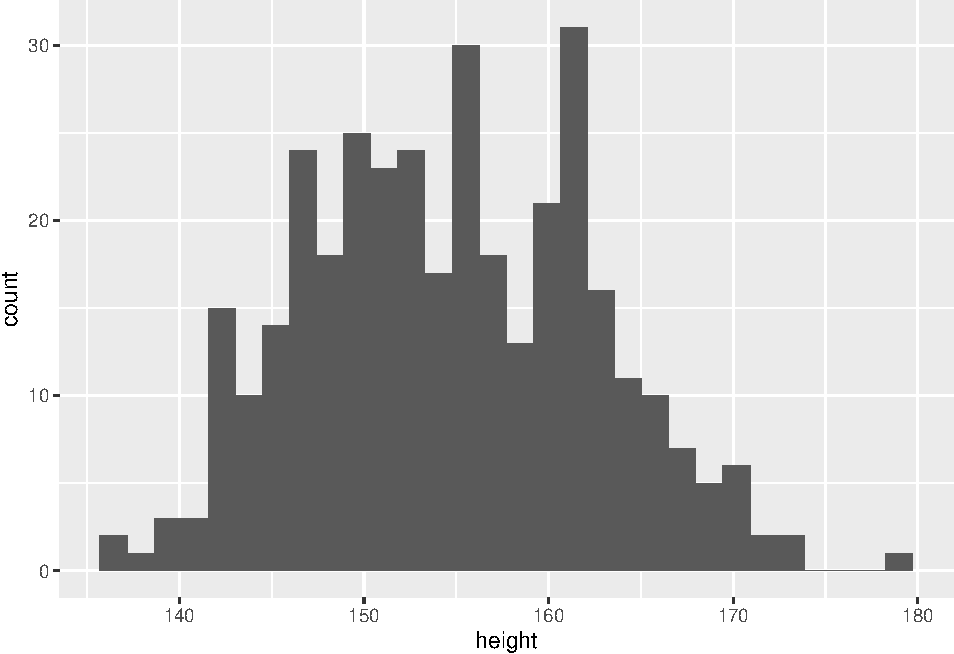
\includegraphics[keepaspectratio]{bookdown-demo_files/figure-latex/unnamed-chunk-2-1.pdf}}

Since we already have domain knowledge in this area, we can say that heights are usually normally distributed,
or at least a mixture of normal distrubutions (female/male).
We assume the following model:
\[h_i \sim \text{Normal}(\mu, \sigma)\]

As in \href{https://jdegenfellner.github.io/Script_QM1_ZHAW/}{QM1},
we want to start with a Bayesian model and hence, we need some priors.

Since we are in Switzerland and just for fun, we use the mean of
\href{https://www.bfs.admin.ch/asset/de/30305714}{Swiss body heights}
as expected value for the \textbf{prior for the mean}.
According to the link (Bundesamt für Statistik),
the mean height of \(n=21,873\) people in the Swiss sample is
\(171.1\) cm. We choose the same \(\sigma\) for the prior of the normal
as in the book not to deviate too much from the example at hand.

Next comes our \textbf{model definition in the Bayesian framework}, which
I often find more intuitive than the frequentist approach:

\[
h_i \sim \text{Normal}(\mu, \sigma)
\]
\[
\mu \sim \text{Normal}(171.1, 20)
\]
\[
\sigma \sim \text{Uniform}(0, 50)
\]

\textbf{Description of the model definition}: The heights are normally distributed with unknown mean and
standard deviation. As our current knowledge about the mean height, we use
a prior distribution for the mean (we do not know but want to estimate) by
assuming the mean of a population we know and a standard deviation of \(20\) cm which
allows are rather large range of possible values for \(\mu\).
\(\sigma\) is also unknown and a priori we restrict ourselves to values
between \(0\) and \(50\) cm, whereas we assign equal plausibility to all
values in this range (which can and should be critically discussed).

\textbf{Vizualisation of the model structure}:
\pandocbounded{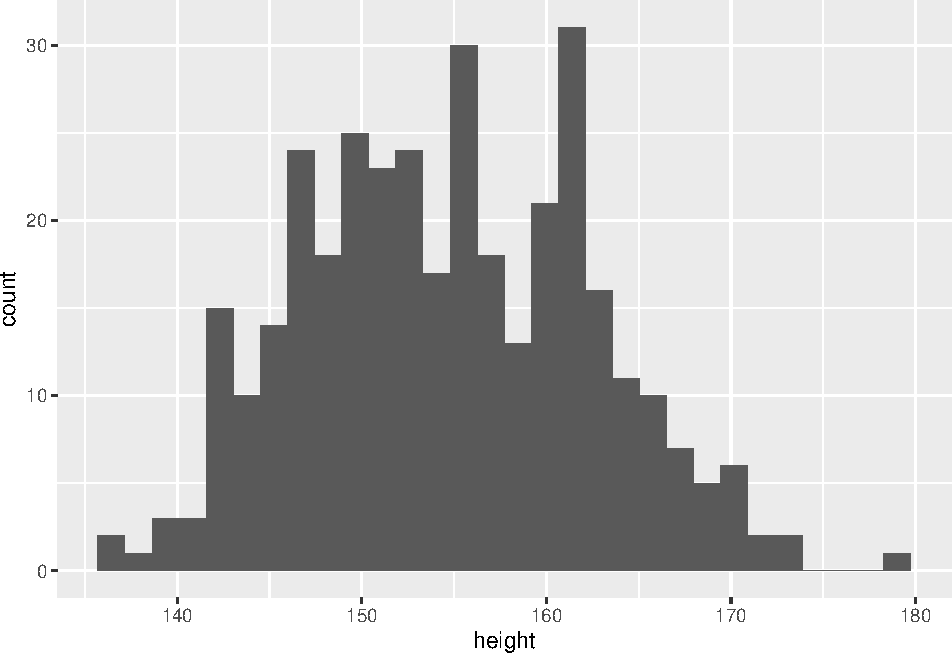
\includegraphics[keepaspectratio]{bookdown-demo_files/figure-latex/unnamed-chunk-3-1.pdf}}

Mind that there is a conceptual difference between the normal distribution of the heights
and the normal prior distribution of the mean. The latter expresses our prior knowledge/insecurity
about the unobserved mean. The normal distribution says we expect the heights to be normally distributed
but we do not know the parameters (\(\mu\) and \(\sigma\)) yet.

Of course we would not need the prior here due to the large sample size,
but let's do it anyways for demonstration purposes.
We are not completely uninformed about body heights and express our
knowledge with the prior for \(\mu\).
The \(20\) in the prior for the mean expresses our range of possible true
mean values and aknowledge
that there are a variety of different subpopulations with different means.

Using the Swiss data in the link one could estimate that the standard deviation of the heights
from \(21,873\) Swiss people is around is \(25.6553\) cm (\hyperref[exercise1_Intro]{Exercise 1}).

Remember, in the Baysian world, there is no \textbf{fixed but unknown}
parameter, but instead we define a distribution over the unobserved parameter.

We \textbf{visualize the prior for \(\mu\)}.

\begin{Shaded}
\begin{Highlighting}[]
\FunctionTok{curve}\NormalTok{(}\FunctionTok{dnorm}\NormalTok{(x, }\FloatTok{171.1}\NormalTok{, }\DecValTok{20}\NormalTok{), }\AttributeTok{from =} \DecValTok{100}\NormalTok{, }\AttributeTok{to =} \DecValTok{250}\NormalTok{)}
\end{Highlighting}
\end{Shaded}

\pandocbounded{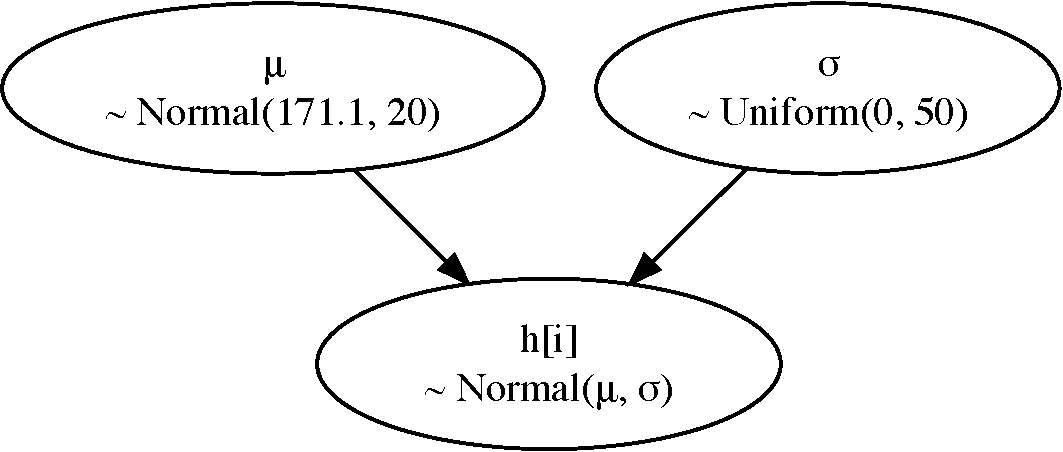
\includegraphics[keepaspectratio]{bookdown-demo_files/figure-latex/unnamed-chunk-4-1.pdf}}

The \textbf{prior for \(\sigma\)} is uniform between \(0\) and \(50\) cm. This is a very wide prior and
just constrains the values to be positive and below \(50\) cm.
This could be stronger of course.

\textbf{Visualization of the prior for \(\sigma\)}:

\begin{Shaded}
\begin{Highlighting}[]
\FunctionTok{curve}\NormalTok{(}\FunctionTok{dunif}\NormalTok{(x, }\DecValTok{0}\NormalTok{, }\DecValTok{50}\NormalTok{), }\AttributeTok{from =} \SpecialCharTok{{-}}\DecValTok{10}\NormalTok{, }\AttributeTok{to =} \DecValTok{60}\NormalTok{)}
\end{Highlighting}
\end{Shaded}

\pandocbounded{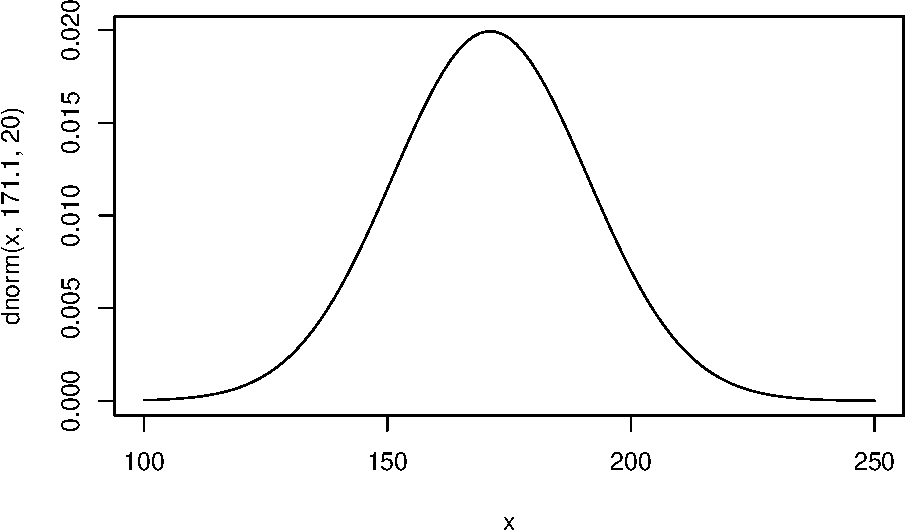
\includegraphics[keepaspectratio]{bookdown-demo_files/figure-latex/unnamed-chunk-5-1.pdf}}

Note, we didn't specify a prior probability distribution of heights
directly, but once we've chosen priors for \(\mu\) and \(\sigma\), these imply a
prior distribution of individual heights.

\textbf{Without} even having seen the \textbf{new data}, we can check what our prior
(model) for heights would predict. This is important. If the prior already
predicts impossible values, we should reconsider our priors and/or model.

So, we simply draw \(\mu\) and \(\sigma\) from the priors and then draw heights
from the normal distribution using the drawn parameters.

\textbf{Vizualisation of the prior for heights}:

\begin{Shaded}
\begin{Highlighting}[]
\NormalTok{sample\_mu }\OtherTok{\textless{}{-}} \FunctionTok{rnorm}\NormalTok{(}\DecValTok{10}\SpecialCharTok{\^{}}\DecValTok{4}\NormalTok{, }\FloatTok{171.1}\NormalTok{, }\DecValTok{20}\NormalTok{)}
\NormalTok{sample\_sigma }\OtherTok{\textless{}{-}} \FunctionTok{runif}\NormalTok{(}\DecValTok{10}\SpecialCharTok{\^{}}\DecValTok{4}\NormalTok{, }\DecValTok{0}\NormalTok{, }\DecValTok{50}\NormalTok{)}
\NormalTok{prior\_h }\OtherTok{\textless{}{-}} \FunctionTok{rnorm}\NormalTok{(}\DecValTok{10}\SpecialCharTok{\^{}}\DecValTok{4}\NormalTok{, sample\_mu, sample\_sigma)}
\FunctionTok{length}\NormalTok{(prior\_h)}
\end{Highlighting}
\end{Shaded}

\begin{verbatim}
## [1] 10000
\end{verbatim}

\begin{Shaded}
\begin{Highlighting}[]
\FunctionTok{dens}\NormalTok{(prior\_h)}
\end{Highlighting}
\end{Shaded}

\pandocbounded{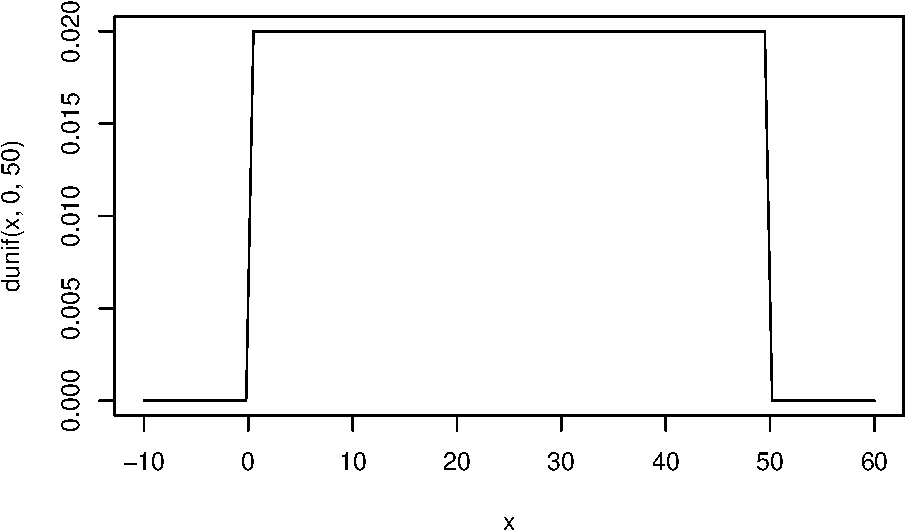
\includegraphics[keepaspectratio]{bookdown-demo_files/figure-latex/unnamed-chunk-6-1.pdf}}

The prior is not itself a Gaussian distribution, but a distribution of
relative plausibilities of different heights, before seeing the data.

Now, there are a couple of different ways to estimtate the model incorporating
the new data. For didactic reasons, grid approximation is often used (as in the book).
For many parameters, grid approximation becomes more and more infeasible (due to combinatorial explosion).

We will skip that for now and use quadratic approximation instead which
works well for many common procedures in applied statistics (like linear regression).
Later, you'll probably use (or the software in the background) mostly Markov
chain Monte Carlo (MCMC) sampling to get the posterior.
\href{https://civil.colorado.edu/~balajir/CVEN6833/bayes-resources/RM-StatRethink-Bayes.pdf}{Pages 39 and the following}
explain the 3 concepts grid approximation, quadratic approximation and MCMC.

In short, \textbf{quadratic approximation} assumes that our posterior distribution
of body heights can be approximated well by a normal distribution,
at least near the peak.

Please read the \hyperref[bivariate_normal]{addendum} to get a clearer picture of
what a bivariate normal distribution is.

Using the library \texttt{rethinking} we can estimate the model using quadratic approximation.
First, we define the model in the \texttt{rethinking} syntax (see R code 4.25 in the book).

\begin{Shaded}
\begin{Highlighting}[]
\FunctionTok{library}\NormalTok{(rethinking)}
\NormalTok{flist }\OtherTok{\textless{}{-}} \FunctionTok{alist}\NormalTok{(}
\NormalTok{  height }\SpecialCharTok{\textasciitilde{}} \FunctionTok{dnorm}\NormalTok{(mu, sigma),}
\NormalTok{  mu }\SpecialCharTok{\textasciitilde{}} \FunctionTok{dnorm}\NormalTok{(}\FloatTok{171.1}\NormalTok{, }\DecValTok{20}\NormalTok{),}
\NormalTok{  sigma }\SpecialCharTok{\textasciitilde{}} \FunctionTok{dunif}\NormalTok{(}\DecValTok{0}\NormalTok{, }\DecValTok{50}\NormalTok{)}
\NormalTok{)}
\end{Highlighting}
\end{Shaded}

Then we estimate/fit the model using quadratic approximation.

\begin{Shaded}
\begin{Highlighting}[]
\NormalTok{m\_heights }\OtherTok{\textless{}{-}}\NormalTok{ rethinking}\SpecialCharTok{::}\FunctionTok{map}\NormalTok{(flist, }\AttributeTok{data =}\NormalTok{ d2)}
\end{Highlighting}
\end{Shaded}

Now let's take a look at the fit \emph{maximum a posteriori} model:

\begin{Shaded}
\begin{Highlighting}[]
\FunctionTok{precis}\NormalTok{(m\_heights)}
\end{Highlighting}
\end{Shaded}

\begin{verbatim}
##             mean        sd       5.5%      94.5%
## mu    154.604128 0.4119929 153.945684 155.262572
## sigma   7.731307 0.2913835   7.265619   8.196994
\end{verbatim}

Above, we see the mean of the posterior for \(\mu\) \textbf{and} \(\sigma\);
and a 89\% credible interval for those parameters.

We can now plot the posterior distribution of the mean and the standard deviation.

\begin{Shaded}
\begin{Highlighting}[]
\NormalTok{post }\OtherTok{\textless{}{-}} \FunctionTok{extract.samples}\NormalTok{(m\_heights, }\AttributeTok{n =} \DecValTok{10}\SpecialCharTok{\^{}}\DecValTok{4}\NormalTok{)}
\FunctionTok{head}\NormalTok{(post)}
\end{Highlighting}
\end{Shaded}

\begin{verbatim}
##         mu    sigma
## 1 154.3276 7.719313
## 2 154.1342 7.740430
## 3 154.7665 7.716517
## 4 154.8177 7.389127
## 5 154.1811 7.526809
## 6 154.3403 7.971658
\end{verbatim}

\begin{Shaded}
\begin{Highlighting}[]
\FunctionTok{dens}\NormalTok{(post}\SpecialCharTok{$}\NormalTok{mu)}
\end{Highlighting}
\end{Shaded}

\pandocbounded{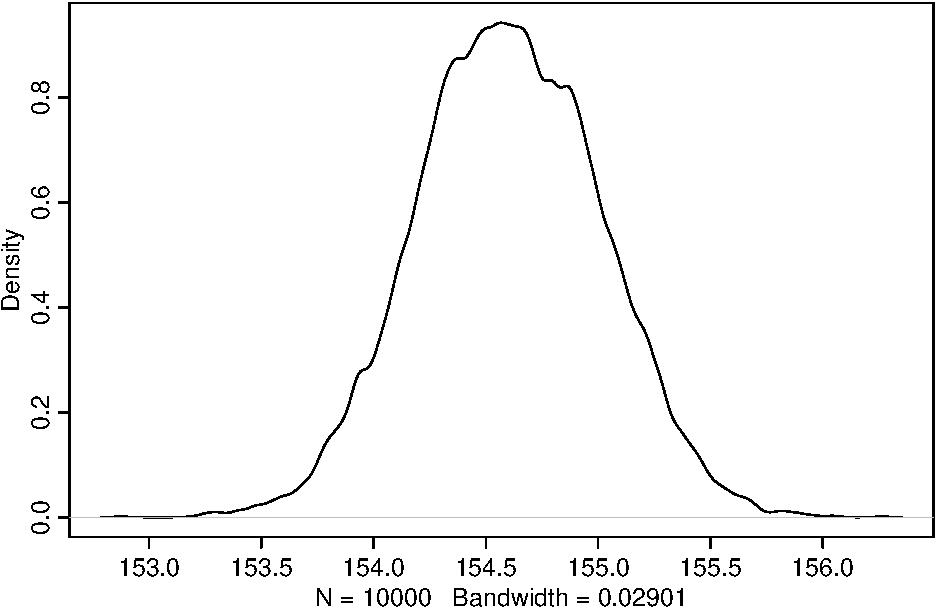
\includegraphics[keepaspectratio]{bookdown-demo_files/figure-latex/unnamed-chunk-10-1.pdf}}

\begin{Shaded}
\begin{Highlighting}[]
\FunctionTok{dens}\NormalTok{(post}\SpecialCharTok{$}\NormalTok{sigma)}
\end{Highlighting}
\end{Shaded}

\pandocbounded{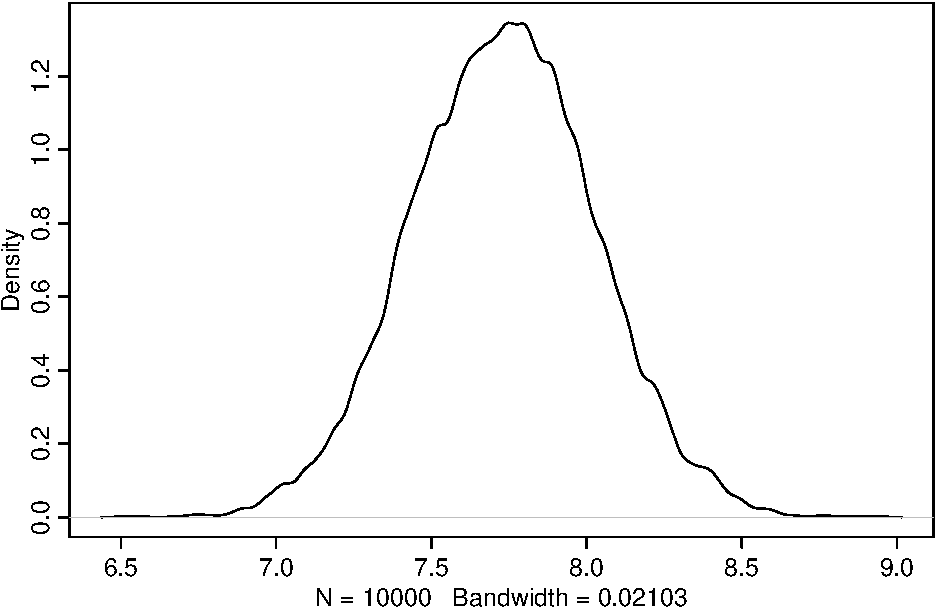
\includegraphics[keepaspectratio]{bookdown-demo_files/figure-latex/unnamed-chunk-10-2.pdf}}

Note, that \textbf{these samples come from a multi-dimensional posterior distribution}.
In our case, we approximated the posterior with a
\href{https://en.wikipedia.org/wiki/Multivariate_normal_distribution}{bivariate normal distribution}.
They are not necessarily independent from each other, but in this case they are.
We know this from the model definition above. \(\mu\) and \(\sigma\) are both
defined as normal respectively uniform distributions and by definition do not
influence each other. This is also visible in the vizualisation of the model structure:
There is no confounding variable or connection between those priors. One could
think of a common variable \(Z\) that influences both \(\mu\) and \(\sigma\). This could
be genetic similarity which could influence both \(\mu\) and \(\sigma\).

Let's verify that \(\mu\) and \(\sigma\) are uncorrelated:

\begin{Shaded}
\begin{Highlighting}[]
\FunctionTok{vcov}\NormalTok{(m\_heights)}
\end{Highlighting}
\end{Shaded}

\begin{verbatim}
##                 mu        sigma
## mu    0.1697381561 0.0001544557
## sigma 0.0001544557 0.0849043302
\end{verbatim}

gives you the variance-covariance matrix of the parameters of the posterior
distribution. In the diagonal you see the variance of the parameters.

\begin{Shaded}
\begin{Highlighting}[]
\FunctionTok{diag}\NormalTok{(}\FunctionTok{vcov}\NormalTok{(m\_heights))}
\end{Highlighting}
\end{Shaded}

\begin{verbatim}
##         mu      sigma 
## 0.16973816 0.08490433
\end{verbatim}

And we can compute the correlation matrix easily:

\begin{Shaded}
\begin{Highlighting}[]
\FunctionTok{cov2cor}\NormalTok{(}\FunctionTok{vcov}\NormalTok{(m\_heights))}
\end{Highlighting}
\end{Shaded}

\begin{verbatim}
##                mu       sigma
## mu    1.000000000 0.001286617
## sigma 0.001286617 1.000000000
\end{verbatim}

Let's plot the posterior in 3D, because we \textbf{can}:

\pandocbounded{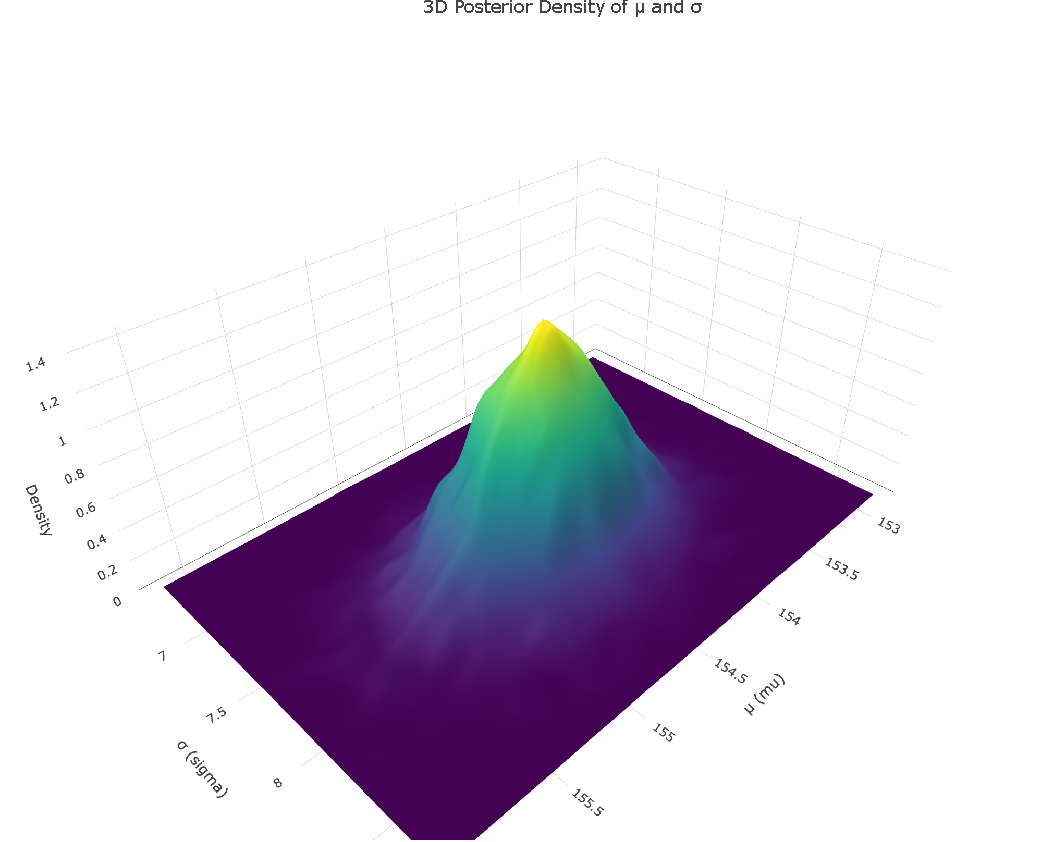
\includegraphics[keepaspectratio]{bookdown-demo_files/figure-latex/posterior-3d-correct-1.pdf}}

\textbf{How beautiful ist that?}

We see in the 3D plot, that the ``mountain'' is not rotated, indicating
graphically that the parameters are independent from each other.

We also see in the correlation matrix, the correlation of the parameters is \(\sim 0\).
In the \href{https://en.wikipedia.org/wiki/Correlation\#Correlation_and_independence}{context of a joint normal distribution},
this means that the parameters are independent.

And, it is not an accident that the posterior looks like this. Using quadratic approximation,
we used the bivariate normal distribution to \textbf{approximate} the posterior.

\section{Exercises}\label{exercises}

\subsection{{[}E{]} Exercise 1}\label{exercise1_Intro}

Use the \href{https://www.bfs.admin.ch/asset/de/30305714}{Swiss body heights} data to
determine
- the 95\% ``Vertrauensintervall'' for \(\mu\) and
- calculate the standard deviation of the heights from \(21,873\) Swiss people.

\section{Addendum}\label{addendum}

\subsection{The bivariate normal distribution}\label{bivariate_normal}

As a refresher, you can look into the old QM1 script and read the
chapter ``4.7 Gemeinsame Verteilungen''.
Maybe \href{https://www.youtube.com/watch?v=SP2GKq8xJ5I&ab_channel=StatisticsNinja}{this video}
also helps.

The bivariate normal distribution is a generalization of the normal distribution to two dimensions.
Now, we look at the distribution of two random variables \(X\) and \(Y\) \textbf{at the same time}.

Instead of one Gaussian bell curve, we have a
\href{https://en.wikipedia.org/wiki/Multivariate_normal_distribution\#/media/File:Multivariate_Gaussian.png}{3D bell curve}.
This curve defines how plausible different combinations of \(X\) and \(Y\) are.

Single points (like (3,6)) still have probability zero, because now the \textbf{volume} over a single point
(\(x\), \(y\)) is zero. The probability of a certain area is now the \textbf{volume} under the
curve compared to the \textbf{area} under the density curve in the one-dimensional case.

\textbf{Example}: The following plot shows the density of a bivariate normal distribution of
two variables \(X\) and \(Y\)
with \(\mu_X = 0\), \(\mu_Y = 0\), \(\sigma_X = 1\), \(\sigma_Y = 1\) and \(\rho = \frac{2}{3}\).

Below is the correlation matrix of the bivariate normal distribution.

\begin{verbatim}
##           [,1]      [,2]
## [1,] 1.0000000 0.6666667
## [2,] 0.6666667 1.0000000
\end{verbatim}

\pandocbounded{
\includegraphics[keepaspectratio]{bookdown-demo_files/figure-latex/unnamed-chunk-14-1.pdf}}

If you move the plot around with your mouse, you see that there is a positive
correlation between \(X\) and \(Y\) (\(\rho = \frac{2}{3}\)). This means that if \(X\) is
above its mean, \(Y\) is also more likely to be above its mean.
The variances of \(X\) and \(Y\) are both \(1\). That means, that if you cut
through the plot in \(X=0\) or \(Y=0\), you see the same form of normal distribution.
If you look at if from above, we have hihglighted the section on the surface
over the area \(X \in [0.5, 2]\) and \(Y \in [0.5, 2]\). The volume over this area
under the density curve is the probability of this area: \(P(X \in [0.5, 2] \text{ and } Y \in [0.5, 2])\)

\chapter{Literature}\label{literature}

Here is a review of existing methods.

\chapter{Methods}\label{methods}

We describe our methods in this chapter.

Math can be added in body using usual syntax like this

\section{math example}\label{math-example}

\(p\) is unknown but expected to be around 1/3. Standard error will be approximated

\[
SE = \sqrt{\frac{p(1-p)}{n}} \approx \sqrt{\frac{1/3 (1 - 1/3)} {300}} = 0.027
\]

You can also use math in footnotes like this\footnote{where we mention \(p = \frac{a}{b}\)}.

We will approximate standard error to 0.027\footnote{\(p\) is unknown but expected to be around 1/3. Standard error will be approximated

  \[
  SE = \sqrt{\frac{p(1-p)}{n}} \approx \sqrt{\frac{1/3 (1 - 1/3)} {300}} = 0.027
  \]}

\chapter{Applications}\label{applications}

Some \emph{significant} applications are demonstrated in this chapter.

\section{Example one}\label{example-one}

\section{Example two}\label{example-two}

\chapter{Final Words}\label{final-words}

We have finished a nice book.

\bibliography{book.bib,packages.bib}

\end{document}
